\documentclass[../paper.tex]{subfiles}
\begin{document}
\section{Recognition}
\label{sec:recognition}

\subsection{Data Collection and Augmentation}

\subsubsection*{Source of Data}
The success of any machine learning project is heavily dependent on the quality and quantity of the data collected. To create a robust data set, we sourced approximately 250,000 images of ASL fingerspelling from three publicly accessible Kaggle data sets \cite{Kaggle1, Kaggle2, Kaggle3}. These images covered the full spectrum of ASL alphabets, ensuring that the model could accurately recognize each letter in different hand positions and varying distances from the camera. The diversity of these images was crucial to account for the variability in real-world scenarios. Additionally, we removed training data for the dynamic letters $\mathbf{\{J, Z\}}$ as their fingerspelling involve movement, which would require a separate model to recognize.

\begin{figure}[!htbp]
  \centerline{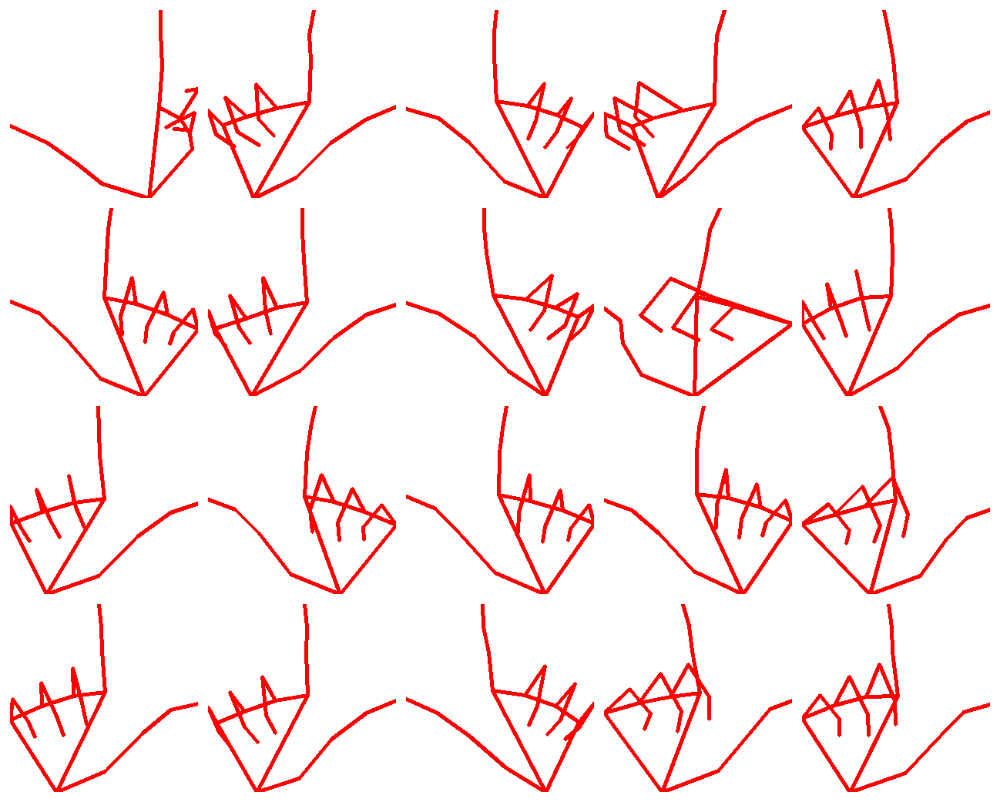
\includegraphics[width=\linewidth]{../figures/net-gallery.png}}
  \caption{Processed training data for the letter \lq L\rq}\label{fig:net_gallery}
\end{figure}

\subsubsection*{Preprocessing}
To ensure that the model maintained accuracy regardless of variability and to ensure it functioned in real-time, the data was converted to Google MediaPipe \cite{MediaPipe} hand landmarks and stored as NumPy \cite{numpy} arrays. This processing reduced the size of the data set to approximately 150,000 images where MediaPipe could accurately detect the 21 landmarks. Then, the detected landmarks were also scaled and normalized to a common reference frame, ensuring consistency across different images. Overall, the use of Google MediaPipe and the utilized normalization techniques made the data invariant to varying backgrounds, lighting conditions, skin tones, hand sizes, and distances from the camera. \autoref{fig:net_gallery} shows a visualized sample of the processed training data for the letter \lq L\rq.

\subsection{Model Training}

As seen in \autoref{fig:recognition_training}, we use the augmented data set to train two classification models: a custom 2D convolutional classification model and an implementation of the 3D PointNet architecture \cite{PointNet}. The custom 2D convolutional classification model was built for simplicity and speed, while the 3D PointNet model was more complex but provided better accuracy.

\begin{figure}[!htbp]
  \centerline{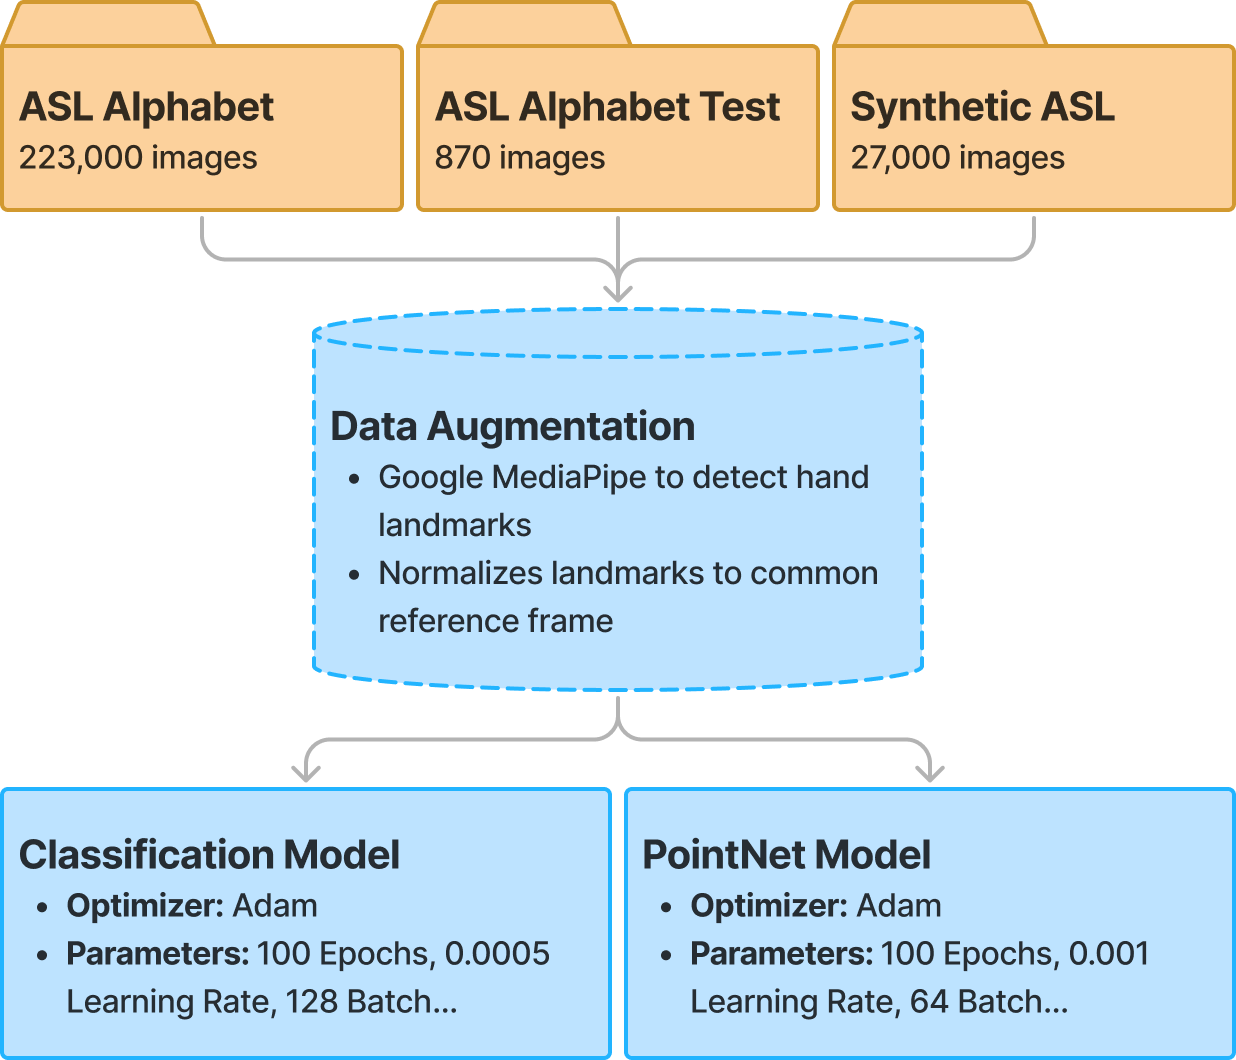
\includegraphics[width=\linewidth]{../figures/recognition-training.png}}
  \caption{Recognition training flow}\label{fig:recognition_training}
\end{figure}

\subsubsection*{2D CNN Architecture}

The custom 2D convolutional classification model was built using the TensorFlow Keras API \cite{tensorflow,keras}. For this implementation, we ignore the z-dimension of the MediaPipe hand landmarks to reduce the complexity of the model. The model features two convolutional blocks, each consisting of two ReLU convolutional layers with a max pooling layer and a batch normalization layer. The output of the second convolutional block is flattened and fed into a set of dense and dropout layers prior to softmax activation. The model was trained using the Adam optimizer with a learning rate of 0.0005 and a sparse categorical cross-entropy loss function. It was trained for 100 epochs with a batch size of 128, achieving a training and validation accuracy of 99.67\% and 99.89\% respectively. \autoref{fig:cnn_architecture} illustrates the model architecture.

\begin{figure}[!htbp]
  \centerline{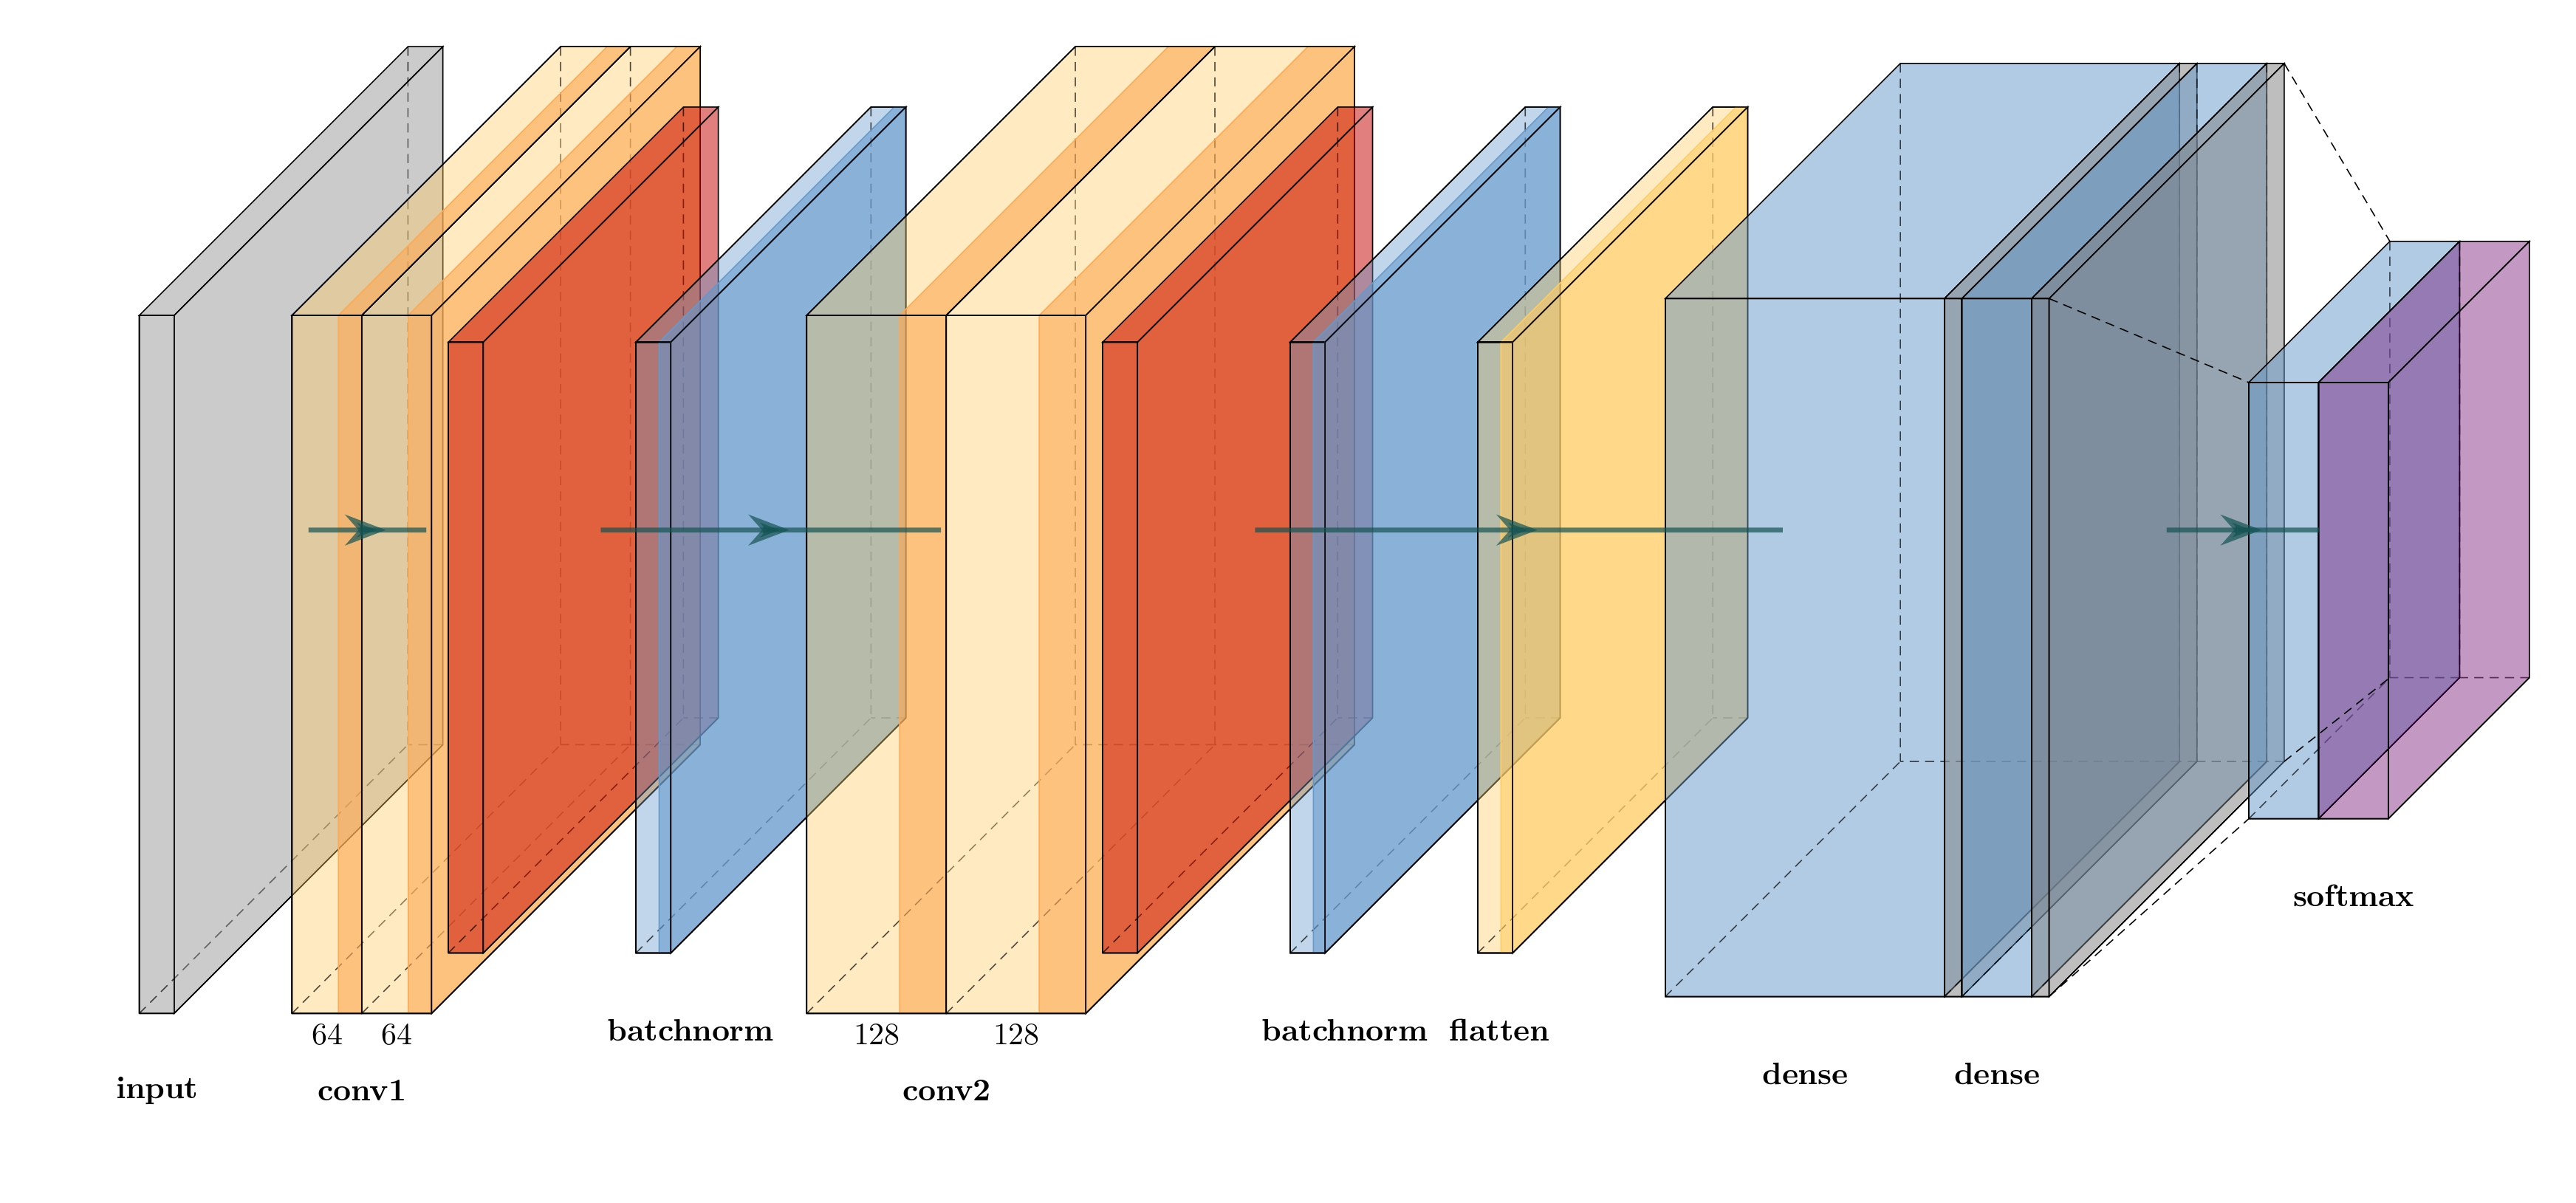
\includegraphics[width=\linewidth]{../figures/recognition-architecture.jpg}}
  \caption{Custom CNN architecture}\label{fig:cnn_architecture}
\end{figure}

\subsubsection*{PointNet Architecture}

 PointNet \cite{PointNet} provides a point cloud classification architecture that is invariant to permutations, rotations, and translations of the input data. The model uses a series of multi-layer perceptrons (MLPs) to transform the input point cloud into a higher-dimensional feature space and then aggregates the features using max pooling layers. Then, it uses softmax activation to create a probability distribution over the output classes.

 \begin{figure}[!htbp]
  \centerline{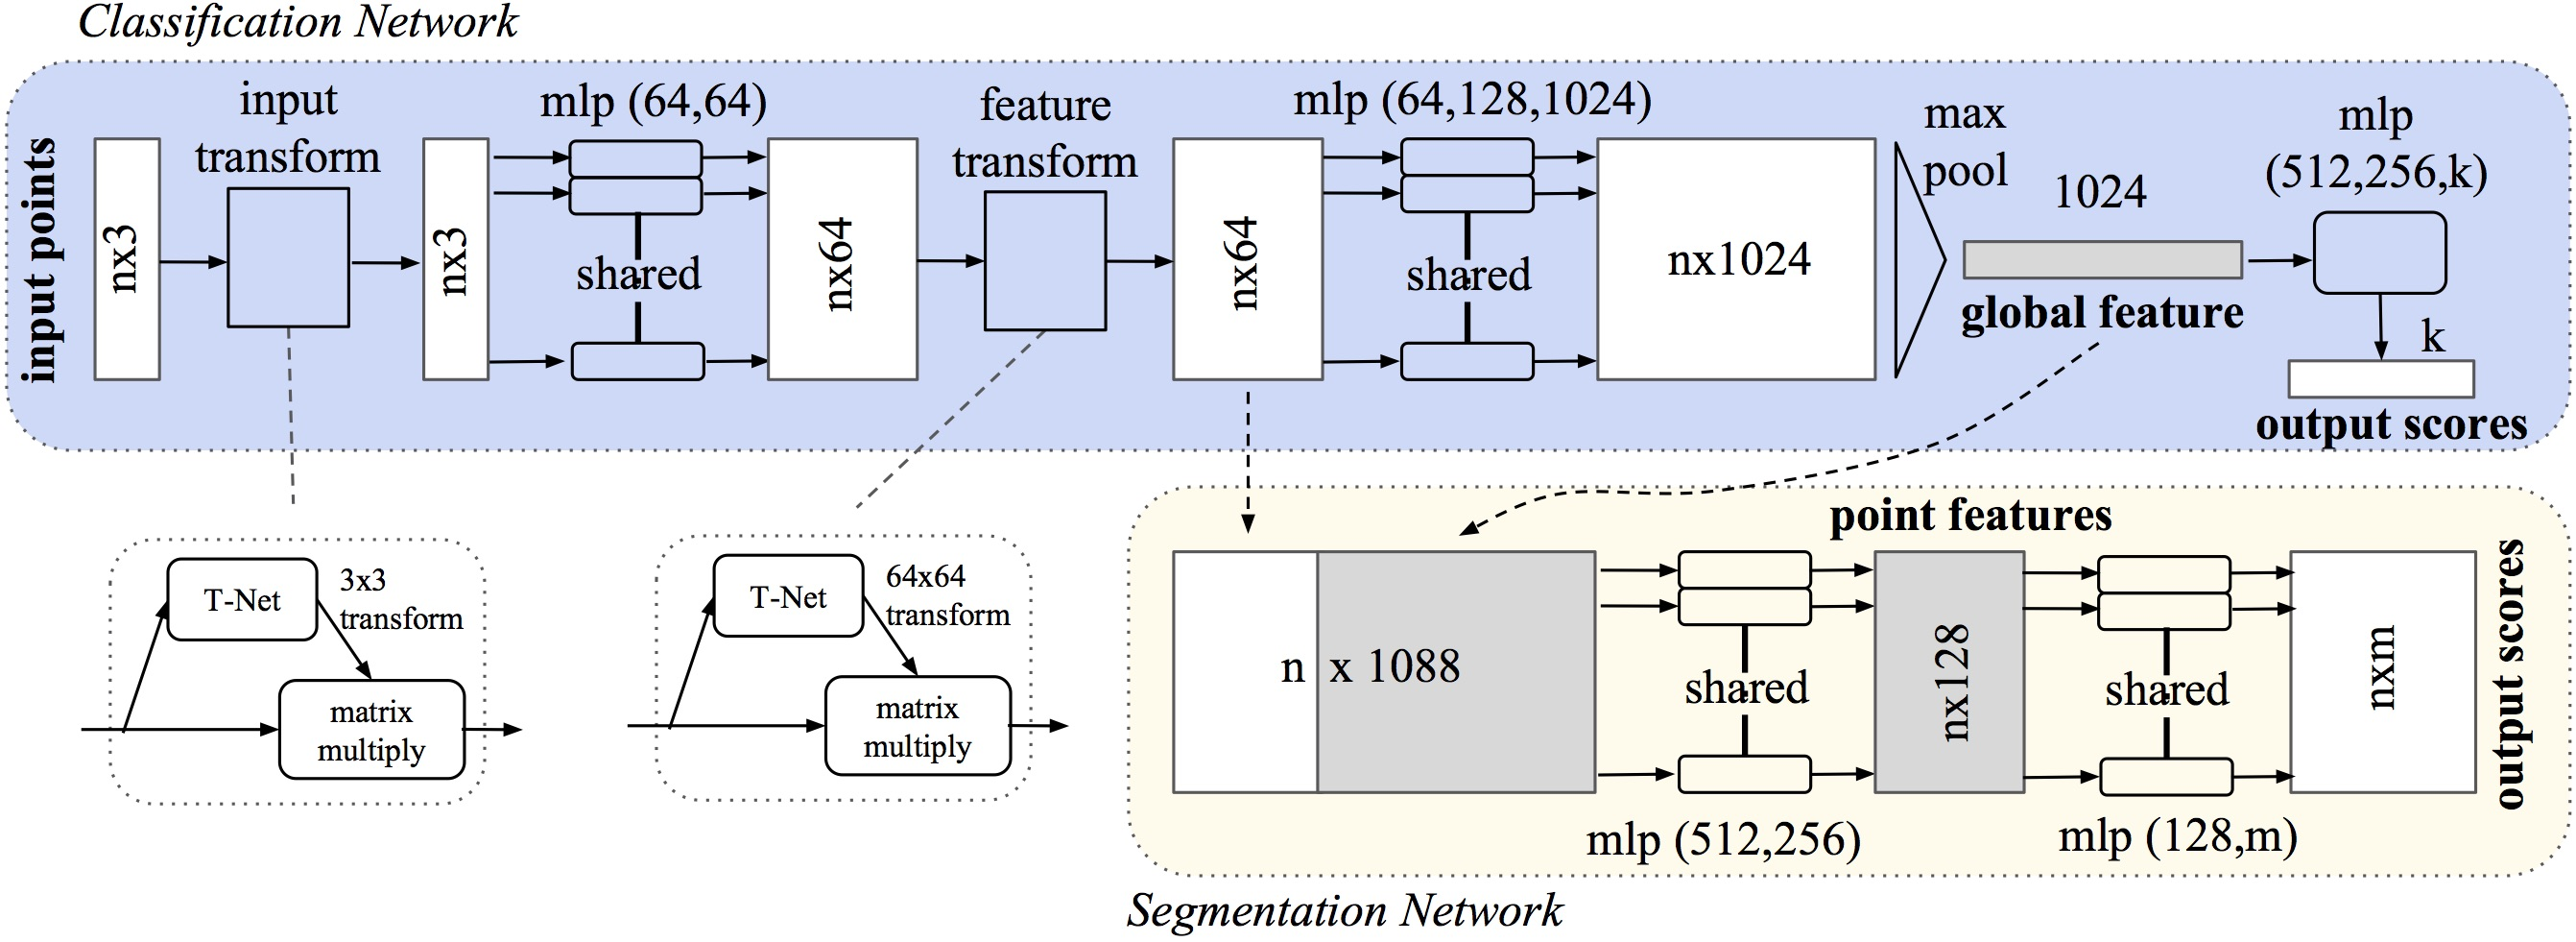
\includegraphics[width=\linewidth]{../figures/pointnet-architecture.jpg}}
  \caption{PointNet Architecture}\label{fig:pointnet_architecture}
\end{figure}

 We implemented the 3D PointNet architecture using the TensorFlow Keras API \cite{tensorflow,keras}. The model was trained using the Adam optimizer with a learning rate of 0.0005 and a sparse categorical cross-entropy loss function. It was trained for 100 epochs with a batch size of 64, achieving a training and validation accuracy of 99.39\% and 99.43\% respectively. \autoref{fig:pointnet_architecture} illustrates the complete PointNet architecture.

\subsection{Model Inference}
The inference stage of the model includes three main steps: fingerspelling-to-landmark conversion, landmark-to-text classification, and text synthesis. \autoref{fig:recognition_flow} demonstrates the complete inference architecture of the recognition component of the interface.


\subsubsection*{Fingerspelling \textrightarrow\ Landmark Conversion}
The Google MediaPipe Hand Landmark model is used to detect 21 landmarks in the inputted frames. The detected landmarks are then scaled and normalized to a common reference frame, ensuring consistency across different images, and making the model invariant to hand sizes and distances from the camera. Now, since the system is only dealing with the 21 landmarks, the computational resources required to run the model are significantly reduced, allowing for real-time fingerspelling recognition in real-world scenarios.
\subsubsection*{Landmark \textrightarrow\ Text Classification}
The normalized landmarks from the previous step are fed into either the 2D CNN model or the 3D PointNet model. The models classify the fingerspelling into individual letters, and the output is a sequence of English alphabets. We ensure that every fingerspelled letter is present over multiple consecutive frames to reduce the likelihood of misclassification. Furthermore, we use conditionals to differentiate between commonly misrecognized letters. For instance, since the letters $\mathbf{\{A, M, N, S, T\}}$ are commonly misrecognized, we use conditionals to distinguish the position of key landmarks like the thumb to correct these misclassifications.
\subsubsection*{Text Synthesis}
We insert a space between words when the hand is not present in the frame, and we prevent the repetition of the same letter more than twice consecutively. Finally, we use a pretrained BERT model to correct syntactical misclassifications and grammar errors. Overall, this process ensures that the model can accurately recognize fingerspelling and synthesize it into coherent spoken English text.

\begin{figure}[!htbp]
  \centerline{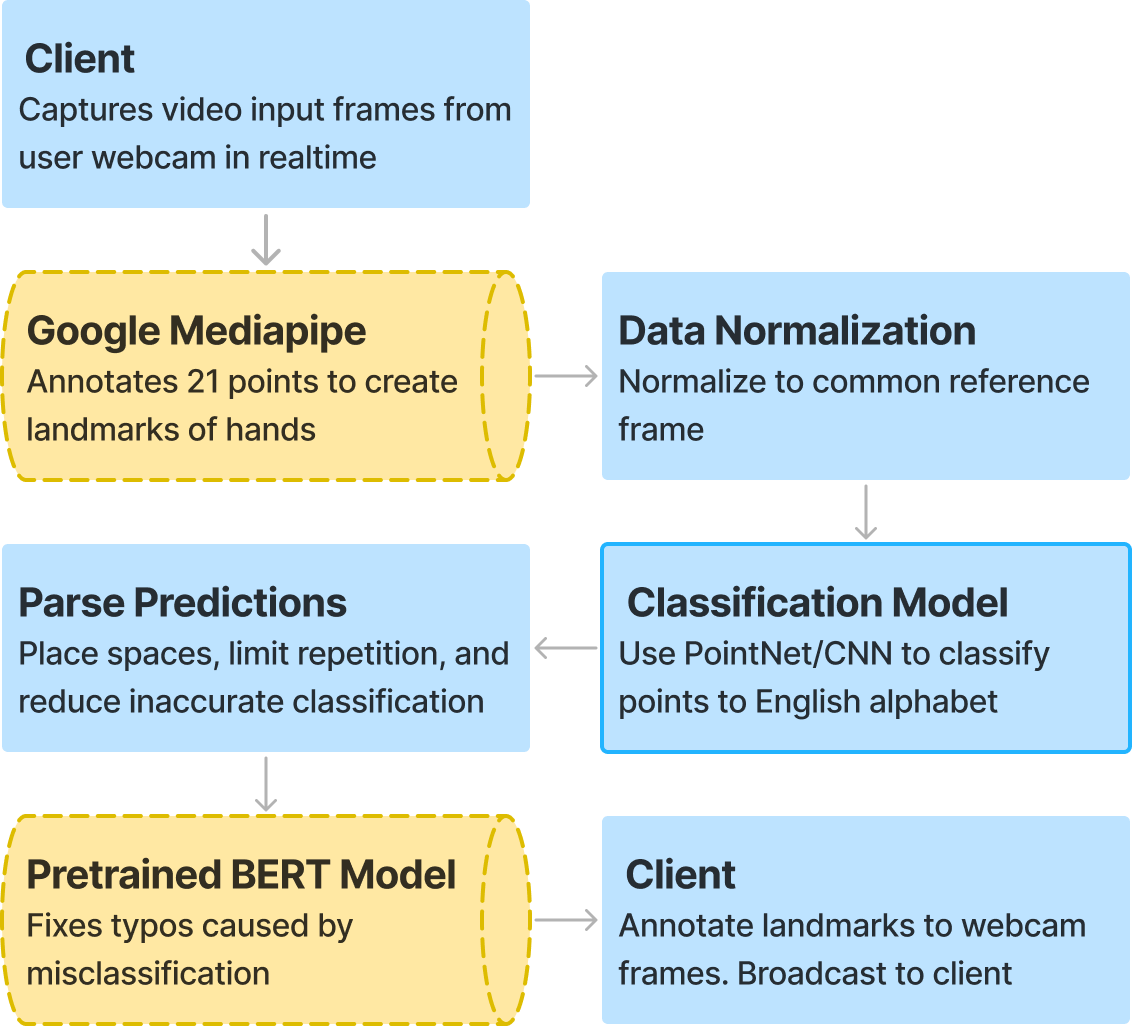
\includegraphics[width=\linewidth]{../figures/recognition-flow.png}}
  \caption{Recognition infrastructure}\label{fig:recognition_flow}
\end{figure}

\end{document}